\documentclass{amsart}
\usepackage[margin=3cm]{geometry}                % See geometry.pdf to learn the layout options. There are lots.
\geometry{letterpaper}                   % ... or a4paper or a5paper or ...
%\geometry{landscape}                % Activate for for rotated page geometry
\usepackage[parfill]{parskip}    % Activate to begin paragraphs with an empty line rather than an indent
\usepackage{float}
\usepackage{graphicx}
\usepackage{amssymb}
\usepackage{epstopdf}
\usepackage{siunitx}
\usepackage{subcaption}
\usepackage{units}
\usepackage{setspace}

\DeclareGraphicsRule{.tif}{png}{.png}{`convert #1 `dirname #1`/`basename #1 .tif`.png}
\graphicspath{{./img/}}

\title{Photoelectric Effect}
\author{Caspar \textsc{Lant}} % Author name

\date{\today} % Date for the report

\begin{document}

\bigskip

\maketitle % Insert the title, author and date
\begin{center}

Intermediate Experimental Physics II\\
\vspace{1.5cm}

\begin{tabular}{l r}

Section: & 001\\
\\
Date Performed: & March 15, 2016 \\ % Date the experiment was performed
Date Due: & March 22, 2016\\
\\
Partner: & Neil Saddler\\ % Partner names
Professor: & Prof. Andrew Kent\\
Instructor: & David Mykytyn % Instructor/supervisor
\end{tabular}
\vfill
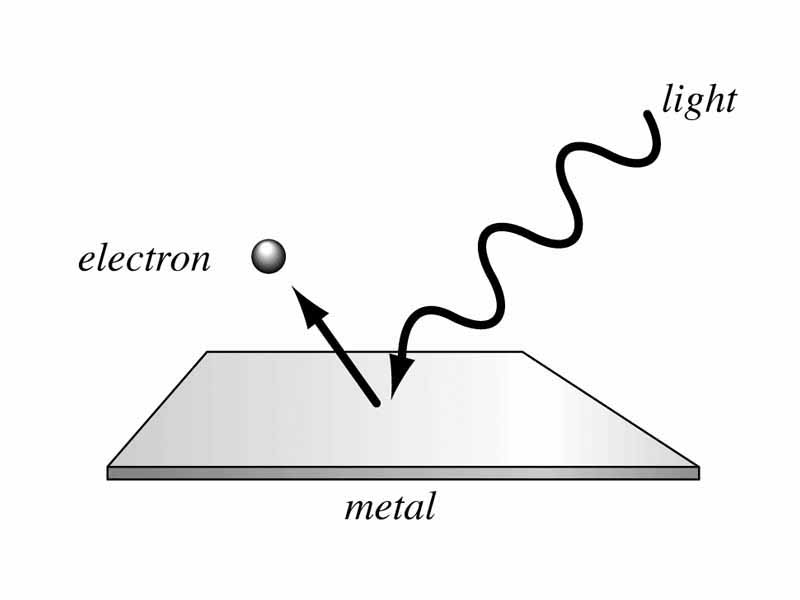
\includegraphics[width=.7\textwidth]{diagram.jpg}
\end{center}
\vfill
\pagebreak

\setstretch{1.5}
\paragraph{\textbf{The Objective} of this lab was to observe the famous photoelectric effect first hand, and to experimentally derive the value of Planck's constant, a quantity central to the study of quantum physics.   }

\section{Theoretical Background/ Abstract}
As we know, it is largely the electrostatic attractive force that keeps electrons from zooming away from their respective atomic nuclei. The strong and week forces are responsible for keeping an atom's nucleus intact, and keeping orbiting electrons from ``falling" into the nucleus of an atom. It was not until the beginning of the 20th century that Albert Einstein, a well known scientist at the time, theorized that the energy of these orbiting electrons was quantized, following the discovery of the photoelectric effect. This was seen as a discovery important enough to land him a Nobel Prize, which is a well-respected distinction in the field of Physics, and relatively hard to come by. The photoelectric effect is best described as the observation that many metals emit electrons when light shines upon them, to quote the popular and often-right web encyclopedia, Wikipedia. What's interesting about the photoelectic effect, that disagrees with a classical interpretation of physics, is the fact that, for a given material, incident light below a certain frequency will not ``bounce off" any photoelectrons, regardless of its intensity. It is only after this frequency threshold (known as the threshold frequency) that higher intensity light produces more photoelectrons. Yes, this means that one can give an object charge by putting it in the path of some high-frequency light. The energy of a photon is given by its frequency times Planck's constant, or $E = h\nu$. Don't ask my why the Greek letter is used in this case instead of the typical `f', but quantum physicists seem to like it, and they tend to know what they're doing. There's another quantity, which we call the work function, given by $\phi = h\nu_0$, where $h$ is Plank's constant again, and $\nu_0$ is the threshold frequency. The kinetic energy of a photoelectron is equal to it's energy minus the work function, which represents the work that it had to do to free itself from the parent material.
\begin{equation}
    K_{max} = h\nu - \phi
\end{equation}
If we take $V_S$, the stopping potential, to be the kinetic energy of a given photoelectron times its charge, we can produce the following equation:
\begin{equation}
    V_s = \dfrac{h}{\rm e} \nu - \dfrac{\phi}{\rm e}
\end{equation}
From here, we can find Plank's constant---assuming that we know the charge of an electron, $e$, and can collect a set of stopping voltages for an array of frequencies of incedent light---as it is the slope.

\section{Experimental Procedure}
\begin{enumerate}
    \item Plug everything in in the manner depicted in the schematic.
    \item Now that I know that you don't read the procedure section, typing them up has become so much more laborious.
    \item Put on your pair of Ali-G glasses and instruct your partner to do the same.
    \item Remember, always don your pair of glasses first if your partner is unable to do so.
    \item Turn on the Ammeter (referred to in the lab manual as a galvenometer) and zero it.
    \item Zero both potentiometers such that the retarded voltage (displayed on the multimeter) is zero volts.
    \item Turn on the UV lamp and place it close to the device's aperture. Wait a minute and note the deflection on the ammeter.
    \item Turn the dial photoelectric effect device to the 577 nm wavelength position.
    \item Record the ammount of deflection by the ammeter for retarding voltages of zero to three volts, at tenth-of-a-volt intervals.
    \item Turn the dial to the next setting and repeat the last 3 steps.
    \item Repeat the last three steps for the remaining two wavelengths.
\end{enumerate}

\section{Graphs and Tables}

\begin{table}[H]
    \begin{minipage}{.45\textwidth}
\centering
\caption{Voltage vs. Deflection}
\bigskip \bigskip
\label{my-label}
\begin{tabular}{c|c|c|c}
Voltage (V) & 546nm & 577nm & 435nm \\ \hline
0.0         & 22.0  & 4.9   & 60.5  \\
0.1         & 16.0  & 3.3   & 47.8  \\
0.2         & 10.1  & 2.0   & 33.9  \\
0.3         & 5.0   & 0.9   & 21.5  \\
0.4         & 1.7   & 0.1   & 11.7  \\
0.5         & -0.1  & 0.0   & 4.0   \\
0.6         & -0.9  & 0.0   & -1.2  \\
0.7         & -1.2  & 0.0   & -5.0  \\
0.8         & -1.3  & 0.0   & -7.5  \\
0.9         & -1.4  & 0.0   & -9.0  \\
1.0         & -1.4  & 0.0   & -10.0 \\
1.1         & -1.5  & 0.0   & -10.5 \\
1.2         & -1.5  & 0.0   & -10.9 \\
1.3         & -1.5  & 0.0   & -11.0 \\
1.4         & -1.5  & 0.0   & -11.1 \\
1.5         & -1.5  & 0.0   & -11.1 \\
1.6         & -1.5  & 0.0   & -11.1 \\
1.7         & -1.5  & 0.0   & -11.1 \\
1.8         & -1.5  & 0.0   & -11.1 \\
1.9         & -1.5  & 0.0   & -11.1 \\
2.0         & -1.5  & 0.0   & -11.1 \\
2.1         & -1.5  & 0.0   & -11.2 \\
2.2         & -1.5  & 0.0   & -11.2 \\
2.3         & -1.5  & 0.0   & -11.2 \\
2.4         & -1.5  & 0.0   & -11.2 \\
2.5         & -1.5  & 0.0   & -11.3 \\
2.6         & -1.5  & 0.0   & -11.3 \\
2.7         & -1.5  & 0.0   & -11.3 \\
2.8         & -1.5  & 0.0   & -11.3 \\
2.9         & -1.5  & 0.0   & -11.4
\end{tabular}
\end{minipage}
%
\begin{minipage}{.5\textwidth}
    \centering
    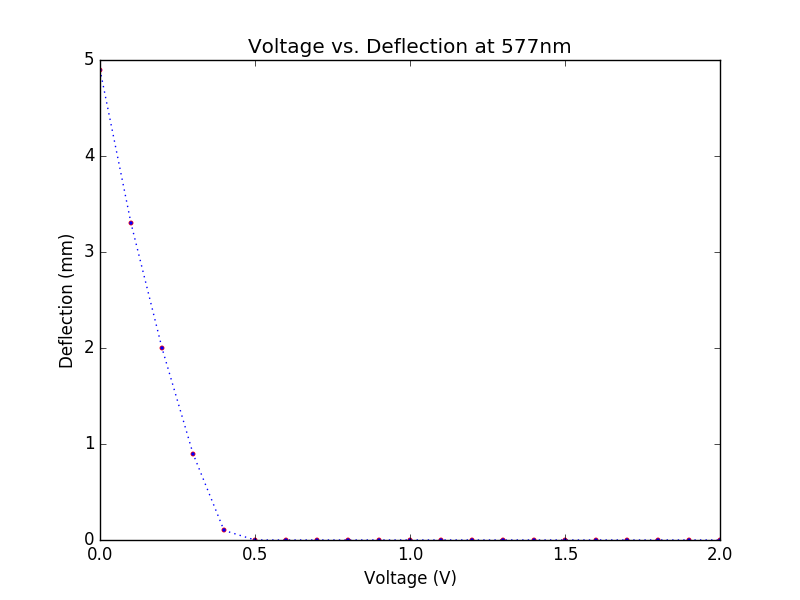
\includegraphics[height=.23\textheight]{577.png}\\
    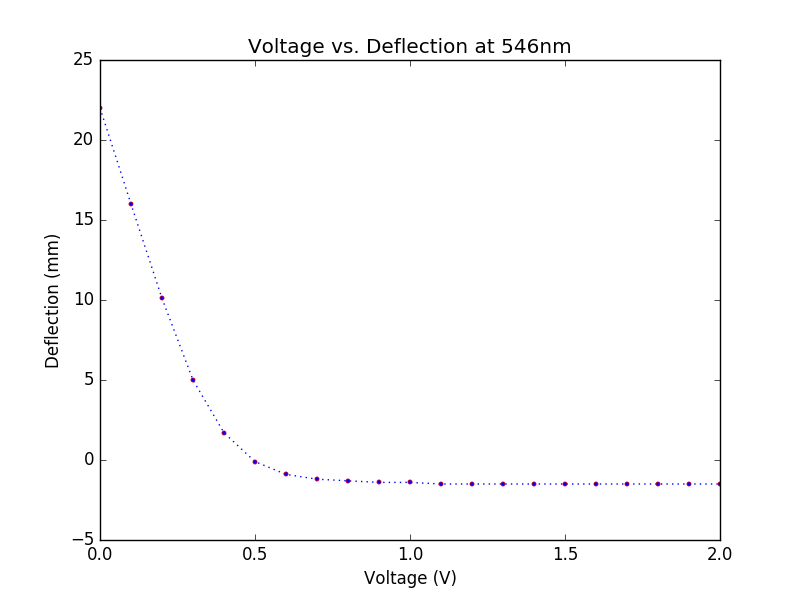
\includegraphics[height=.23\textheight]{546.png}\\
    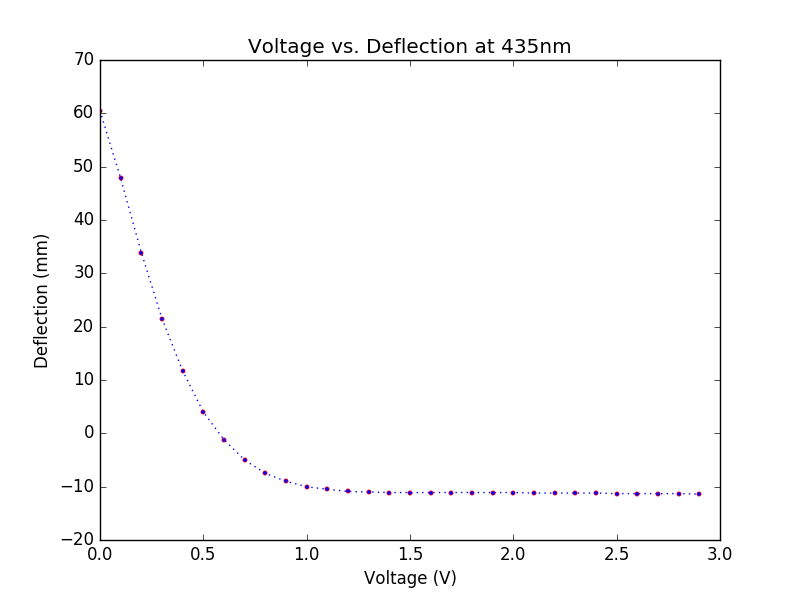
\includegraphics[height=.23\textheight]{435.png}
\end{minipage}
\end{table}

\begin{figure}
    \centering
    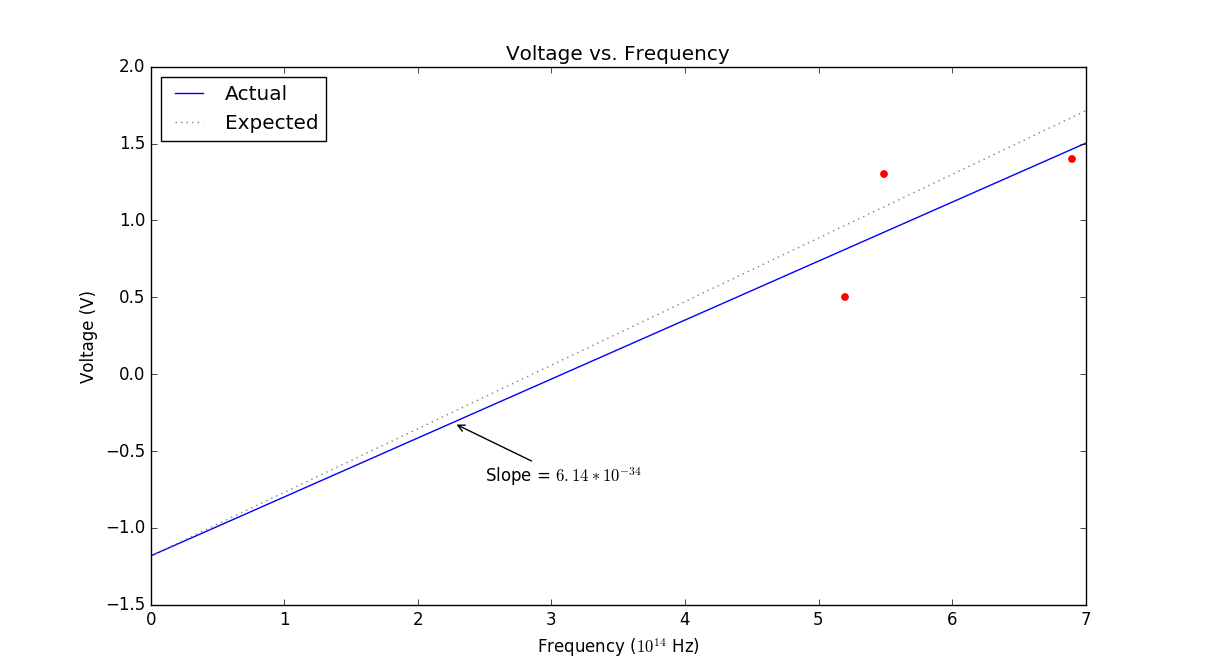
\includegraphics[width=\textwidth]{planckbest.png}
    \caption{Finding Planck's Constant}
    {$h = \unitfrac[6.14 \times 10^{-34}]{ m^2 kg}{s}$}
\end{figure}

\begin{figure}
    \centering
    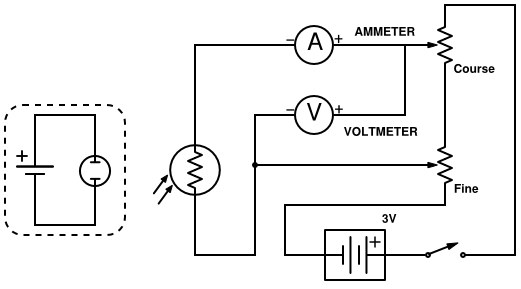
\includegraphics[width=0.8\textwidth]{schematic.png}
    \caption{Schematic Diagram of the Experimental Setup}
\end{figure}


\begin{figure}
    \begin{minipage}{.45\textwidth}
        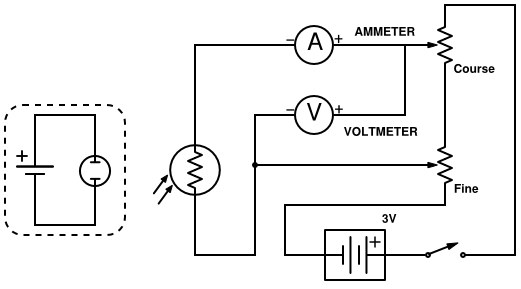
\includegraphics[width=\textwidth]{schematic.png}
    \end{minipage}
    %
    \begin{minipage}{.45\textwidth}

    \end{minipage}
\end{figure}

The topmost plot corresponds to a filter of slit width 577 nm, the middle plot 546 nm, and the last plot a wavelength of 435 nm.
\section{Questions}

\begin{enumerate}
    \item {\textit{Are there any questions to answer in this lab report?}
\begin{quote}
There don't seem to be any questions to answer in this lab report.
\end{quote}}

\end{enumerate}

\section{Error Analysis}




\end{document}
